\chapter{差分法}
\thispagestyle{empty}

\section{差分格式}
设函数$u(x)$定义在一维有界空间上。差分求解需要先将\dy[区域离散化]{QYLSH}(类似于采样),得到由节点构成的网格系统,再利用差分格式建立离散方程。

真实的区域由无限个节点构成,因此这里是用有限个节点来近似无限的系统。

由$u(x)$在点$x$处的泰勒展开
\begin{align}
	u(x + h) & = u(x) + u'(x)h + u''(x)\dfrac{h^2}{2} + u'''(x)\dfrac{h^3}{6} + \cdots\\[0.5em]
	u(x - h) & = u(x) - u'(x)h + u''(x)\dfrac{h^2}{2} - u'''(x)\dfrac{h^3}{6} + \cdots
\end{align}
则
\begin{equation}
	\dfrac{u(x+h)-u(x)}{h} = u'(x) + u''(x)\dfrac{h}{2} + u'''(x)\dfrac{h^2}{6} = u'(x) - O(h) \quad \Rightarrow \quad u'(x) = \dfrac{u(x+h)-u(x)}{h}+O(h)
\end{equation}
其中,$o(h)$为$h$的同阶无穷小量\footnote{即$\displaystyle \lim\limits_{h \to 0} \dfrac{O(h)}{h} = C$(常数)余项,$O(h^2)$类似},称为\dy[截断误差]{JDWC}。

同理可得
\begin{equation}
	u'(x) = \dfrac{u(x)-u(x-h)}{h}+O(h)
\end{equation}

忽略无穷小量$o(h)$可得
\begin{align}
	u'(x) &\approx \dfrac{u(x+h)-u(x)}{h}\label{前向差分}\\[0.5em]
	& \approx \dfrac{u(x)-u(x-h)}{h}\label{后向差分}\\[0.5em]
	& \approx \dfrac{u(x+h)-u(x-h)}{2h}\label{中心差分}
\end{align}

公式\eqref{前向差分}称为\dy[前向差分]{QXCF},公式\eqref{后向差分}称为\dy[后向差分]{HXCF},公式\eqref{中心差分}称为\dy[中心差分]{ZXCF}。二阶导数的中心差分为
\begin{equation}
	u''(x) \approx \dfrac{u(x+h)-2u(x)+u(x-h)}{h^2}
\end{equation}


由于前向和后向差分中截断误差为$O(h)$,则前向和后向差分具有一阶精度,中心差分的阶段误差为$O(h^2)$,具有二阶精度。精度越高,误差以越快的速度趋于零,但所需要的信息也越多。

定义\dy[截断误差的阶数]{JDWCDJS}为随着网格尺寸趋于零时,截断误差趋于零的速度,则\textbf{$n$阶精度格式 $=$ 该格式的截断误差为$n$阶}。精度和节点数量是差分法近似程度的两个重要保障,在相同的近似程度下,高精度格式所需的节点数量更少。

差分的形式可以总结表示为
\begin{equation*}
	\mbox{连续区域} \xrightarrow{\scriptsize \quad \mbox{离散化}\quad }\mbox{由节点构成的网络}\xrightarrow{\scriptsize \quad \mbox{四种形式}\quad}\mbox{离散方程}
\end{equation*}
具体的四种形式如表\ref{差分的四种表示形式}.

\begin{table}[!htb]
	\centering
	\setlength{\tabcolsep}{9mm}{
	\begin{tabular}{cccc}
		\toprule
		导数 & 差分格式 & 阶段误差 & 差分形式 \\
		\midrule
		&&&\\[-1em]
		\multirow{4}{*}{$u'(x)$} & $\dfrac{u(x)-u(x-h)}{h}$ & $o(h)$ & 后向差分\\
		&&&\\[-1em]
		& $\dfrac{u(x+h)-u(x)}{h}$ & $o(h)$ & 前向差分\\
		&&&\\[-1em]
		& $\dfrac{u(x+h)-u(x-h)}{2h}$ & $o(h^2)$ & 中心差分\\
		&&&\\
		$u''(x)$ & $\dfrac{u(x+h)-2u(x)+u(x-h)}{h^2}$ & $o(h^2)$ & 中心差分\\
		&&&\\[-1em]
		\bottomrule
	\end{tabular}
	}
\caption{差分的四种表示形式}
\label{差分的四种表示形式}
\end{table}


\section{Laplace方程的差分解法}
二维Laplace方程
\begin{equation}
	\begin{cases}
		\, \dfrac{\partial^2 u}{\partial x^2} + \dfrac{\partial^2 u}{\partial y^2} = 0, &(x,y)\in \Omega\\[0.5em]
		\, u\big|_\Gamma = f(x,y), & (x,y)\in \Gamma
	\end{cases}
\end{equation}
其中,$\Gamma$ 是平面上不规则有界区域$\Omega$的边界。
\vspace*{0.5em}

\subsection{区域离散化}
如图\ref{区域离散化},离散化的目标:用一系列节点$(i,j)$代替原物理域区域,基本步骤为
\vspace*{-0.5em}
\begin{enumerate}[\hspace*{2em} \textbf{步骤} 1 ]
	\item \textbf{不规则区域变为规则区域}\vspace*{-0.5em}
	\item \textbf{将规则区域进一步划分为正方形网格}
\end{enumerate}
\begin{figure}[!htb]
	\centering
	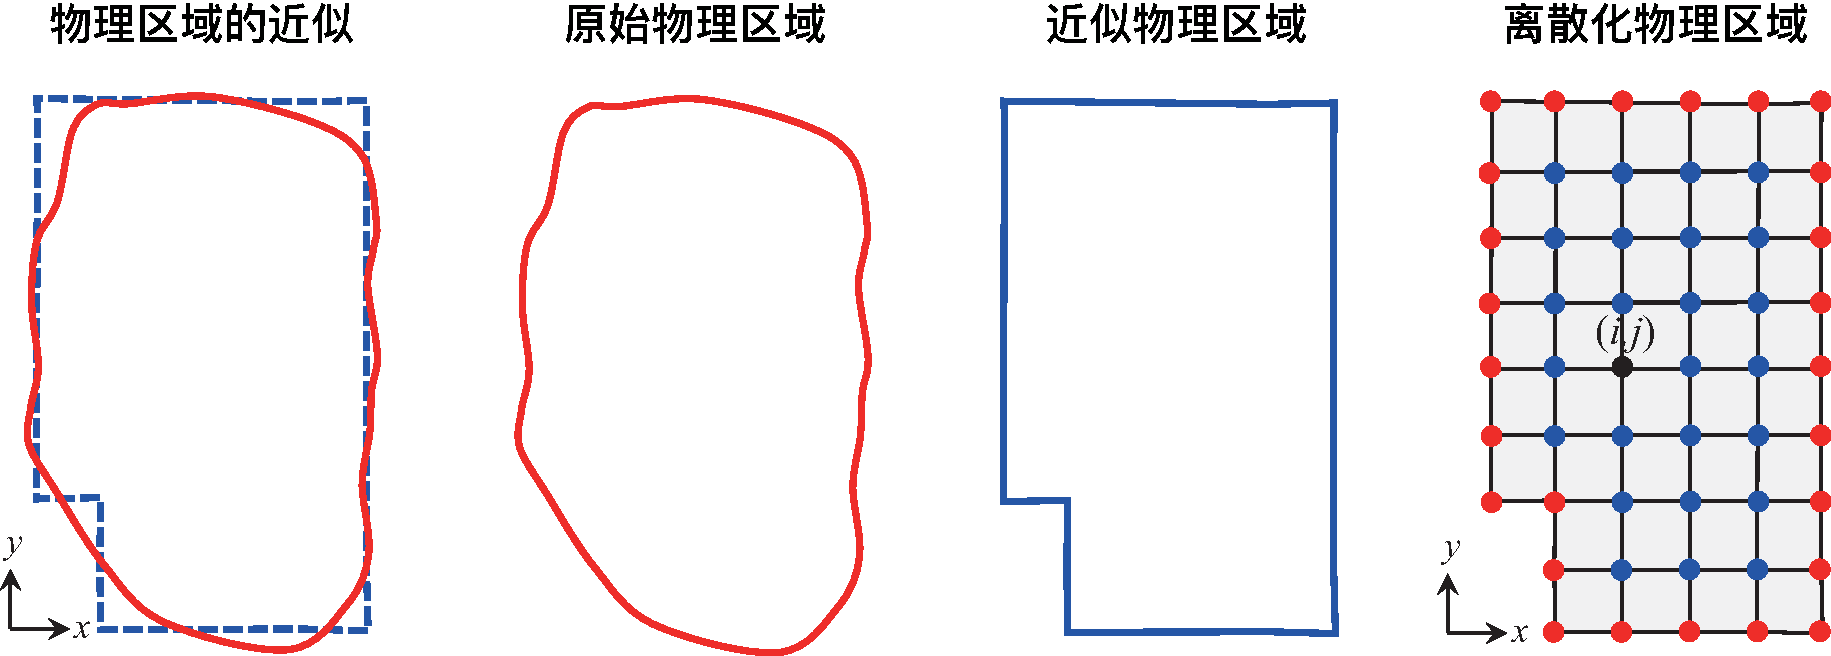
\includegraphics[width=0.85\linewidth]{pic/空间离散化.pdf}
	\caption{区域离散化}
	\label{区域离散化}
\end{figure}
	
离散化以后的区域,网格线的交点、以及网格线与边界的交点称为\dy[节点]{JD} ,用$( i,j)$标记其行和列的位置。红色为边界节点,蓝色为内部节点。正方形网格尺寸$h$称为\dy[节点间距]{JDJJ}。
\vspace*{0.5em}
	
\subsection{建立离散方程}
\begin{itemize}
	\item \textcolor{blue}{内部节点}(蓝色)需要建立离散方程\vspace*{-0.5em}
	\item \textcolor{red}{边界节点}(红色)需赋予相应的边界条件
\end{itemize}
\noindent \textbf{1. 边界条件的指定}

\begin{minipage}{0.7\linewidth}
	\vspace*{1em}
	\begin{itemize}
		\item 在原定解问题中,红色不规则边界上取值已知为$f(x,y)$
		\item 利用$f(x,y)$给定红色边界点上的值
		\item 利用\dy[最近点策略]{ZZDCL},即
		\begin{equation*}
			\mbox{任一红色边界节点的取值}\,=\,\mbox{原红色不规则区域上距离最近的点的取值}
		\end{equation*}
	\end{itemize}

\hspace*{-2em} \textbf{2. 内部节点离散方程的建立}
\vspace*{0.5em}

对于任一内部节点$(i,j)$,由二维Laplace方程可以得到离散方程
\end{minipage}
\begin{minipage}{0.25\linewidth}
	\centering
	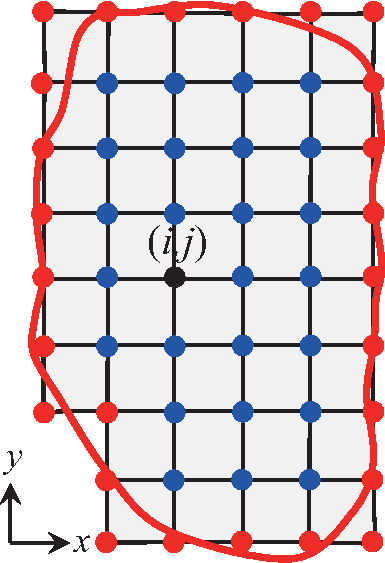
\includegraphics[width=0.8\linewidth]{pic/离散边界.pdf}
	\vspace*{-1em}
	\captionof{figure}{边界条件的指定}
\end{minipage}
\vspace*{0.5em}

\begin{equation}
	\dfrac{\partial^2 u}{\partial x^2} + \dfrac{\partial^2 u}{\partial y^2} \quad \Rightarrow \quad \dfrac{u_{i+1,j} - 2u_{i,j}+u_{i-1,j}}{h^2} + \dfrac{u_{i,j+1}-2u_{i,j}+u_{i,j-1}}{h^2} = 0
\end{equation}
化简得到
\begin{equation}
	u_{i+1,j} + u_{i-1,j} + u_{i,j+1} + u_{i,j-1} -4u_{i,j} = 0
	\label{离散方程}
\end{equation}
即\textcolor{red}{“四周相加,再减四倍”}。公式\eqref{离散方程}对内部所有节点都成立。
\vspace*{0.5em}

将所有离散方程联立得到一个\textbf{线性方程组}
\begin{equation}
	\bm{A}\bm{u}=\bm{B}
\end{equation}
其中,$\bm{A}$为系数矩阵,$\bm{u}$为内部节点未知量组成的列向量,非齐次项$\bm{B}$反映边界条件。
\vspace*{1em}

\noindent \textbf{3. 解线性方程组}

求解线性方程组有逆矩阵法和高斯消元法等成熟的算法,在Matlab里,求解$u$的方法为
\begin{center}
	\lstinline|u = A\B|
\end{center}

\examples \label{7.1}如图\ref{7.1.1}所示,给定矩形离散物理空间和边界条件,采用正方形网格,节点间距为$h =1$ ,求满足Laplace方程的内部节点。
\vspace*{-0.5em}
\begin{figure}[!htb]
	\begin{minipage}{0.5\linewidth}
		\centering
		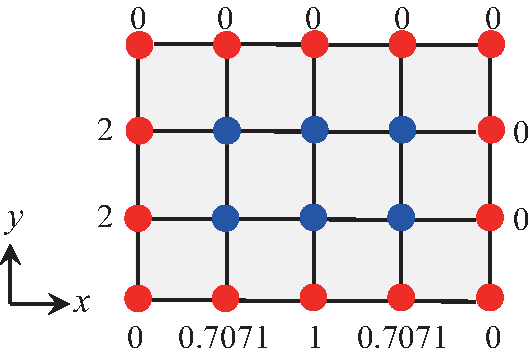
\includegraphics[width=0.6\linewidth]{pic/差分例1-1.pdf}
		\vspace*{-1em}
		\caption{\ref{7.1} $\,$题图}
		\label{7.1.1}
	\end{minipage}
	\begin{minipage}{0.5\linewidth}
		\centering
		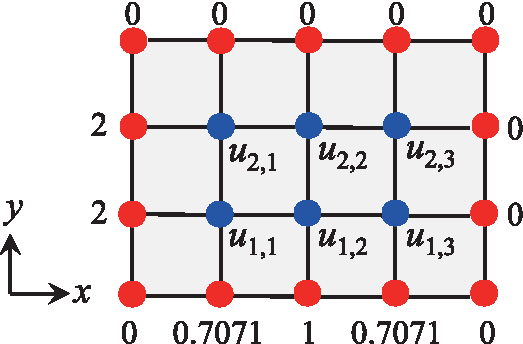
\includegraphics[width=0.6\linewidth]{pic/差分例1-2.pdf}
		\vspace*{-0.6em}
		\caption{\ref{7.1} $\,$编号图}
		\label{7.1.2}
	\end{minipage}
\end{figure}
\vspace*{-0.8em}

\solve 如图\ref{7.1.2}所示,将内部的节点编号,各个点的二阶中心差分离散方程为
\begin{align*}
	(1,1) \quad & u_{2,1} + 2 + 0.7071 + u_{1,2} -4u_{1,1}= 0\\
	(1,2) \quad & u_{2,2} + u_{1,1} + 1 + u_{1,2} -4u_{1,2}= 0\\
	(1,3) \quad & u_{2,3} + u_{1,2} + 0.7071 + 0 -4u_{1,3}= 0\\
	(2,1) \quad & 0 + 2 + u_{1,1} + u_{2,2} -4u_{2,1}= 0\\
	(2,2) \quad & 0 + u_{2,1} + u_{1,2} + u_{2,3} -4u_{2,2}= 0\\
	(2,3) \quad & 0 + u_{2,2} + u_{1,3} + 0 -4u_{2,3}= 0
\end{align*}
得到线性方程组
\begin{equation*}
	\begin{bmatrix}
		-4 & 1 & 0 & 1 & 0 & 0\\
		1& -4 & 1 &  0 & 1 & 0 \\
		0& 1 & -4&  0& 0 & 1\\
		1& 0 & 0 & -4 & 1 & 0\\
		0 & 1 & 0  & 1 & -4 & 1\\
		0& 0& 1 &0 & 0 &-4
	\end{bmatrix}
	\,\,
	\begin{bmatrix}
		u_{1,1}\\
		u_{1,2}\\
		u_{1,3}\\
		u_{2,1}\\
		u_{2,2}\\
		u_{2,3}
	\end{bmatrix}
	\,\,
	=
	\,\,
	\begin{bmatrix}
		-2.7071\\
		-1\\
		-0.7071\\
		-2\\
		0\\
		0
	\end{bmatrix}
\end{equation*}
利用Matlab解得
\begin{equation*}
	\begin{bmatrix}
		u_{1,1}\\
		u_{1,2}\\
		u_{1,3}\\
		u_{2,1}\\
		u_{2,2}\\
		u_{2,3}
	\end{bmatrix}
	\, = \,
	\begin{bmatrix}
		1.0835\\
		0.7405\\
		0.4186\\
		0.8863\\
		0.4616\\
		0.2196
	\end{bmatrix}
\end{equation*}
\vspace*{1em}

\subsection{$\mbox{第三类边界条件的处理}^*$}
上一节仅考虑了第一类边界条件,对于更一般的第三类边界条件的处理如下。
\begin{figure}[!htb]
	\centering
	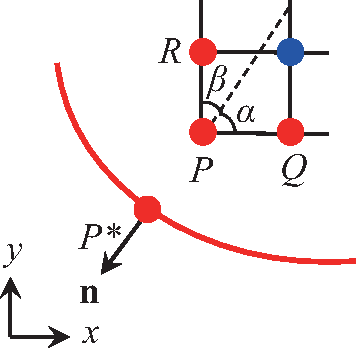
\includegraphics[width=0.2\linewidth]{pic/离散第三边界.pdf}
	\caption{第三边界条件下的边界差分方程}
	\label{第三边界差分}
\end{figure}

如图\ref{第三边界差分},考虑边界上一点$P$,其邻近点记作$Q$和$R$,正方形网格尺寸为$h$,$P$点在真实物理区域上的最近点记作$P^*$.

\noindent 由第三类边界条件,在$P^*$点满足
\begin{equation}
	u(P^*) + \sigma \dfrac{\partial u}{\partial n}\Bigg|_{P^*} = f(P^*)
\end{equation}

\noindent 由最近点方案,可得
\begin{equation}
	u(P) + \sigma \dfrac{\partial u}{\partial n}\Bigg|_{P} = f(P) = f(P^*)
\end{equation}

\noindent 根据几何关系
\begin{equation}
	\dfrac{\partial u}{\partial n}\Bigg|_{P} = - \left(\dfrac{\partial u}{\partial x}\Bigg|_{P} \cos \alpha + \dfrac{\partial u}{\partial y}\Bigg|_{P} \sin \alpha\right)
\end{equation}

\noindent 综合可得
\begin{equation}
	u(P) - \sigma \dfrac{\partial u}{\partial x}\Bigg|_{P}\cos \alpha - \sigma \dfrac{\partial u}{\partial y}\Bigg|_{P} \sin \alpha = f(P^*)
\end{equation}

\noindent 由前向差分的定义
\begin{equation}
	\dfrac{\partial u}{\partial x}\Bigg|_{P} = \dfrac{u(Q) - u(P)}{h}, \quad \dfrac{\partial u}{\partial y}\Bigg|_{P} = \dfrac{u(R) - u(P)}{h}
\end{equation}

\noindent 最终整理得到
\begin{equation}
	[h+\sigma \cos \alpha + \sigma \sin \alpha ]u(P) - (\sigma \cos \alpha)u(Q)-(\sigma \sin \alpha)u(R) = f(P^*)h
	\label{离散第三边界}
\end{equation}

公式\eqref{离散第三边界}仅为\textbf{边界节点值的代数方程},仍需和和内部节点公式\eqref{离散方程}联合组成线性方程组,一并求解。
\vspace*{1em}

\subsection{总结}
 Laplace方程的差分解法总结如下
\begin{enumerate}
	\item \textbf{用一系列离散节点$(i,j)$代替原物理域}
	\item \textbf{处理边界方程,得到离散方程}
	\begin{itemize}
		\item \textbf{第一类边界条件}\quad 对每一内部节点,选取适当的差分格式,得到其离散方程,组成线性方程组
		\item \textbf{第二、第三类边界条件 }\quad 边界条件满足的离散方程将额外给出,和内部节点的方程联立得到线性方程组,其方程数量更多
	\end{itemize}
	\item \textbf{求解线性方程组},得到未知节点处的解,即为原定解问题的近似解。
\end{enumerate}

\warn[
{
\begin{enumerate}
	\item \textbf{网格的形状可以是任意的}\\
	\hspace*{2em}网格不一定是正方形,可以是矩形、平行四边形、三角形、正六边形等等
	\item \textbf{差分格式是多样的}\\
	\hspace*{2em}对于一阶导数,本节介绍了前向、后向、中心差分,对于二阶导数,只介绍了中心差分,然而实际上还有更多更复杂的、精度更高的差分格式
	\item \textbf{线性方程组的求解方法也多种多样}
	\item \textbf{方程还可以含有非齐次项,差分法中称为\dy[源项]{YX}。}所以,这里仅讨论了最简单、最基本的情况。\\[-1em]
\end{enumerate}
}
]
\clearpage

\section{热传导方程的差分解法}
考虑一维热传导方程的简单情况:分析长度为1的杆在$0 \sim T$之间的温度变化,其初始温度为$f(x)$,两端温度固定为0,即
\begin{equation}
	\begin{cases}
		\, \dfrac{\partial u}{\partial t} = a^2 \dfrac{\partial^2 u}{\partial x^2}, & 0<x<1,0<t\le T\\[0.5em]
		\, u\big|_{t=0} = f(x), & 0 \le x \le 1\\
		\, u\big|_{x=0} = u\big|_{x=1} = 0, & 0 < t \le T
	\end{cases}
\end{equation}
\vspace*{0.5em}

\subsection{时间变量的特殊性}
\begin{enumerate}[1. ]
	\item 热传导方程与Laplace方程的不同之处在于,热传导方程是一个\textcolor{red}{非稳态过程},即结果随时间变化的过程。\vspace*{-0.5em}
	\item 非稳态过程的特点是\textcolor{blue}{后一时刻的状态依赖于前一状态},即不能同时知道所有时刻的状态。时间变量必须从$0\sim T$,每一步时间的增量称为\dy[时间步长]{SJBC},记作$\Delta t$.\vspace*{-0.5em}
	\item 求解的过程可以理解为\textcolor{blue}{“基于过去,预测未来”}(随时间向前迭代),其精度与$\Delta t$的长度(步长)相关。
\end{enumerate}

\subsection{建立离散方程}
设空间离散点在某一时刻的状态为$u_i^n$,其中下标$i$表示空间信息,上标$n$表示时间信息。在这里离散成6个等间距节点,其中4 个内部节点,2个边界节点,记节点间距为$h$.如图\ref{一维差分传热}所示。
\begin{figure}[!htb]
	\centering
	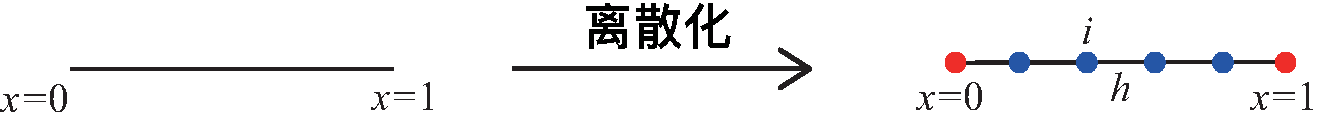
\includegraphics[width=0.6\linewidth]{pic/一维差分传热.pdf}
	\caption{一维传热计算域离散化}
	\label{一维差分传热}
\end{figure}

\noindent \textbf{1. 考虑时间导数项}
\begin{equation*}
	\boxed{\dfrac{\partial u}{\partial t}} = a^2 \dfrac{\partial^2 u}{\partial x^2}
\end{equation*}
\begin{itemize}
	\item 时间导数的差分格式必须要用到下一步的时间信息,才能实现时间推进。由\ptref[差分的四种表示形式]可知只有前向差分和中心差分满足要求。
	\item 这里采用较为简单的前向差分。对目前处于第$n$个时刻的第$i$个内部节点,时间导数项差分后
	\begin{equation}
		\dfrac{u_i^{n+1}-u_i^n}{\Delta t} = a^2 \dfrac{\partial^2 u}{\partial x^2}\Bigg|_i
	\end{equation}
\end{itemize}
\noindent \textbf{2. 考虑空间导数项}
\begin{equation*}
	\dfrac{u_i^{n+1}-u_i^n}{\Delta t} = a^2\,\, \boxed{\dfrac{\partial^2 u}{\partial x^2}\Bigg|_i}
\end{equation*}
\begin{enumerate}[\hspace*{2em} (1) ]
	\item \textbf{显式格式}\\
	当空间导数项采用$n$时刻的空间数据(已知的数据)时,此时可以得到显式方程
	\begin{equation}
		\dfrac{u_i^{n+1}-u_i^n}{\Delta t} = a^2 \dfrac{u_{i+1}^n - 2u_i^n + u_{i-1}^n}{h^2}
	\end{equation}
	从而得到各点的离散方程
	\begin{align*}
		(n,1)\quad &\dfrac{u_1^{n+1}-u_1^n}{\Delta t} = a^2 \dfrac{u_{2}^n - 2u_1^n }{h^2}\\[0.5em]
		(n,2)\quad &\dfrac{u_2^{n+1}-u_2^n}{\Delta t} = a^2 \dfrac{u_{3}^n - 2u_2^n + u_1^n}{h^2}\\[0.5em]
		(n,3)\quad &\dfrac{u_3^{n+1}-u_3^n}{\Delta t} = a^2 \dfrac{u_{4}^n - 2u_3^n + u_2^n}{h^2}\\[0.5em]
		(n,4)\quad &\dfrac{u_1^{n+1}-u_1^n}{\Delta t} = a^2 \dfrac{- 2u_4^n + u_3^n}{h^2}
	\end{align*}
	整理得
	\begin{align}
		\bm{u}^{n+1} = \bm{B}^n
	\end{align}
	其中,
	\begin{equation}
		\bm{u}^{n+1} = 
		\begin{bmatrix}
			\, u_1^{n+1}\, \\
			\, u_2^{n+1}\, \\
			\, u_3^{n+1}\, \\
			\, u_4^{n+1}\,
		\end{bmatrix}
	\quad \quad
	\bm{B}^n = 
	\begin{bmatrix}
		\, u_1^n + a^2 \dfrac{u_{2}^n - 2u_1^n }{h^2}\Delta t \,\\[1em]
		\, u_2^n + a^2 \dfrac{u_{3}^n - 2u_2^n + u_1^n}{h^2} \Delta t \, \\[1em]
		\, u_3^n+a^2 \dfrac{u_{4}^n - 2u_3^n + u_2^n}{h^2}\Delta t \, \\[1em]
		\, u_4^n +a^2 \dfrac{- 2u_4^n + u_3^n}{h^2} \Delta t \, 
	\end{bmatrix}
	\end{equation}
	\vspace*{0.5em}
	
	\item \textbf{隐式格式}\\
	当空间导数项采用$n+1$时刻的空间数据(未知的数据)时,此时可以得到隐式方程
	\begin{equation}
		\dfrac{u_i^{n+1}-u_i^n}{\Delta t} = a^2 \dfrac{u_{i+1}^{n+1} - 2u_i^{n+1} + u_{i-1}^{n+1}}{h^2}
	\end{equation}
	从而得到各点的离散方程
	\begin{align*}
		(n+1,1)\quad &\dfrac{u_1^{n+1}-u_1^n}{\Delta t} = a^2 \dfrac{u_{2}^{n+1} - 2u_1^{n+1} }{h^2}\\[0.5em]
		(n+1,2)\quad &\dfrac{u_2^{n+1}-u_2^n}{\Delta t} = a^2 \dfrac{u_{3}^{n+1} - 2u_2^{n+1} + u_1^{n+1}}{h^2}\\[0.5em]
		(n+1,3)\quad &\dfrac{u_3^{n+1}-u_3^n}{\Delta t} = a^2 \dfrac{u_{4}^{n+1} - 2u_3^{n+1} + u_2^{n+1}}{h^2}\\[0.5em]
		(n+1,4)\quad &\dfrac{u_1^{n+1}-u_1^n}{\Delta t} = a^2 \dfrac{- 2u_4^{n+1} + u_3^{n+1}}{h^2}
	\end{align*}
	整理得
	\begin{align}
		\bm{A}\bm{u}^{n+1} = \bm{B}^n
	\end{align}
	其中,
	\begin{equation}
		\bm{u}^{n+1} = 
		\begin{bmatrix}
			\, u_1^{n+1}\, \\
			\, u_2^{n+1}\, \\
			\, u_3^{n+1}\, \\
			\, u_4^{n+1}\,
		\end{bmatrix}
		\quad \quad
		\bm{B}^n = 
		\begin{bmatrix}
			\, u_1^{n}\, \\
			\, u_2^{n}\, \\
			\, u_3^{n}\, \\
			\, u_4^{n}\,
		\end{bmatrix}
		\quad \quad 
		\bm{A} =
		\begin{bmatrix}
			\, 1+\dfrac{2a^2}{h^2}\Delta t & -\dfrac{a^2}{h^2}\Delta t & 0 & 0\,\, \\[1em]
			\, -\dfrac{a^2}{h^2} \Delta t & 1+\dfrac{2a^2}{h^2}\Delta t & -\dfrac{a^2}{h^2}\Delta t & 0 \,\, \\[1em]
			\, 0 & -\dfrac{a^2}{h^2}\Delta t  & 1+\dfrac{2a^2}{h^2}\Delta t & -\dfrac{a^2}{h^2}\Delta t \,\, \\[1em]
			\, 0 & 0 & -\dfrac{a^2}{h^2}\Delta t  &1+\dfrac{2a^2}{h^2}\Delta t \,\,
		\end{bmatrix}
	\end{equation}
\end{enumerate}
\subsection{时间推进}
\noindent \textbf{1. 显式格式的时间推进}
\begin{figure}[!htb]
	\centering
	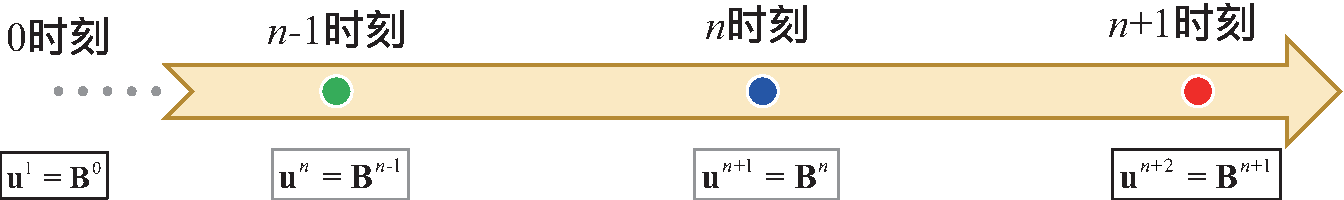
\includegraphics[width=0.7\linewidth]{pic/显式时间.pdf}
	\caption{显式格式的时间推进}
\end{figure}
\vspace*{-2em}

\begin{itemize}
	\item $n$从0开始递增,直到$t=T$为止。
	\item 在每一时刻,只需进行代数运算获得$\bm{B}^n$便得$\bm{u}^{n+1}$,计算量小。
	\item 然而,\textcolor{red}{显式格式的时间步长要很小},否则很容易出现解振荡发散的现象。
\end{itemize}
\vspace*{1em}

\noindent \textbf{2. 隐式格式的时间推进}
\begin{figure}[!htb]
	\centering
	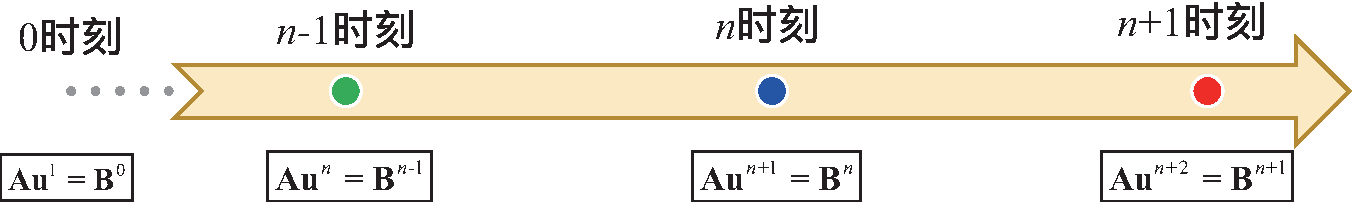
\includegraphics[width=0.7\linewidth]{pic/隐式时间.pdf}
	\caption{隐式格式的时间推进}
\end{figure}
\vspace*{-2em}

\begin{itemize}
	\item $n$从0开始递增,直到$t=T$为止。
	\item 在每一时刻,需求解线性方程组,计算量较大。
	\item 与此同时,\textcolor{red}{允许时间更大的时间步长}。
\end{itemize}

\examples \label{7.2} 考虑长为4的一维杆的热传导问题。已将杆离散为5个节点构成的网格,节点间距$h=1$,内节点标记为$u_1,u_2,u_3$.杆的初始温度和边界温度固定为0,如图\ref{7.2.1}所示。已知热扩散系数$a_2=1$,取时间步长$\Delta t=0.1$,用显式差分法求$t=0.2$时的温度场近似解。
\begin{figure}[!htb]
	\centering
	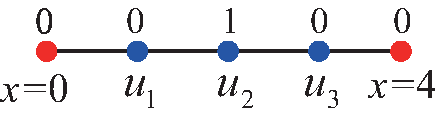
\includegraphics[width=0.24\linewidth]{pic/7.2.1.pdf}
	\vspace*{-0.8em}
	\caption{\ref{7.2}$\,$题图}
	\label{7.2.1}
\end{figure}
\vspace*{-1.5em}

\solve 根据显式有限差分,将方程离散为
\begin{equation*}
	\dfrac{u_i^{n+1}-u_i^n}{\Delta t} = a^2 \dfrac{u_{i+1}^{n+1} - 2u_i^{n+1} + u_{i-1}^{n+1}}{h^2}
	\quad \Rightarrow \quad
	u_i^{n+1} = u_i^n + 0.1\big(u_{i+1}^n -2u_i^n + u_{i-1}^n\big)
\end{equation*}
然后进行时间推进,即将$n=0,\,\,i=1,2,3$代入,得到$t=0.1$时刻的节点值满足
\begin{equation*}
	\begin{aligned}
		u_1^1 &= u_1^0 + 0.1\big(u_2^0 - 2u_1^0 + u_0^0\big)\\
		u_2^1 &= u_2^0 + 0.1\big(u_3^0 - 2u_2^0 +u_1^0\big)\\
		u_3^1 &= u_3^0 + 0.1\big(u_4^0 - 2u_3^0 + u_2^0\big)
	\end{aligned}
	\quad \quad \xrightarrow[\mbox{边界条件}]{\quad \mbox{代入初始条件} \quad} \quad \quad 
	\begin{aligned}
		u_1^1 &= 0+0.1(1-0+0)=0.1\\
		u_2^1 &= 1+0.1(0-2+0)=0.8\\
		u_3^1 &= 0 + 0.1(0-0+1)=0.1
	\end{aligned}
\end{equation*}
得到$t=0.1$时刻的节点值如图\ref{7.2.2}.
\begin{figure}[!htb]
	\centering
	\begin{minipage}{0.4\linewidth}
		\centering
		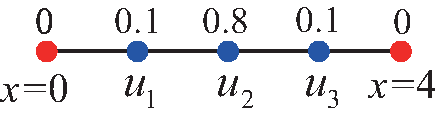
\includegraphics[width=0.6\linewidth]{pic/7.2.2.pdf}
		\vspace*{-0.8em}
		\caption{$t=0.1$时刻的节点值}
		\label{7.2.2}
	\end{minipage}
	\begin{minipage}{0.4\linewidth}
		\centering
		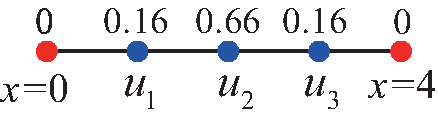
\includegraphics[width=0.6\linewidth]{pic/7.2.3.pdf}
		\vspace*{-0.5em}
		\caption{$t=0.2$时刻的节点值}
		\label{7.2.3}
	\end{minipage}
\end{figure}

继续将$n=1,\,\,i=1,2,3$代入,得到$t=0.2$时刻的节点值满足
\begin{equation*}
	\begin{aligned}
		u_1^2 &= u_1^1 + 0.1\big(u_2^1 - 2u_1^1 + u_0^1\big)\\
		u_2^2 &= u_2^1 + 0.1\big(u_3^1 - 2u_2^1 +u_1^1\big)\\
		u_3^2 &= u_3^1 + 0.1\big(u_4^1 - 2u_3^1 + u_2^1\big)
	\end{aligned}
	\quad \quad \xrightarrow[\mbox{边界条件}]{\quad \mbox{代入新的初始条件} \quad} \quad \quad 
	\begin{aligned}
		u_1^2 &= 0.1+0.1(0.8-2\times 0.1 +0)=0.16\\
		u_2^2 &= 0.8+0.1(0-2\times 0.8+0.1)=0.66\\
		u_3^2 &= 0.1 + 0.1(0-2\times 0.1+0.8)=0.16
	\end{aligned}
\end{equation*}
得到$t=0.2$时刻的节点值如图\ref{7.2.3}.
\vspace*{0.5em}

\subsection{总结}
总结如图\ref{非稳态热传导差分解法总结}所示。
\begin{figure}[!htb]
	\centering
	\begin{tikzpicture}
		\node (A) [inner sep = 6pt, draw] {\makecell[c]{热传导方程同时含有\textcolor{blue}{时间导数}和\textcolor{blue}{空间导数},\\
		由非稳态问题的特点,求解需采用\textcolor{red}{时间推进策略}}};
		\node (B) [inner sep =6pt, draw, below of = A, node distance = 3cm, xshift = -4cm]{\textcolor{blue}{时间导数项$\dfrac{\partial u}{\partial t}$}};
		\node (B1) [inner sep =6pt, draw, below of = B, node distance = 2cm]{时间变量的特殊性:\textcolor{red}{向前不向后}};
		\node (B2) [inner sep = 6pt, draw, below of = B1, node distance = 2.5cm]{$\dfrac{u_i^{n+1}-u_i^n}{\Delta t} = a^2 \dfrac{\partial^2 u}{\partial x^2}\Bigg|_i$};
		
		\node (C) [inner sep =6pt, draw, below of = A, node distance = 3cm, xshift = 4cm]{\textcolor{blue}{空间导数项$\dfrac{\partial^2 u}{\partial x^2}\Bigg|_i$}};
		\node (C1) [inner sep =6pt, draw, below of = C, node distance = 2cm]{采用二阶中心差分,考虑\textcolor{red}{时间的选取}};
		\node (C11) [inner sep =6pt, draw, below of = C1, node distance = 2.2cm, xshift = -2.5cm]{显式格式};
		\node (C111) [inner sep =6pt, draw, below of = C11, node distance = 1.5cm]{$\bm{u}^{n+1} = \bm{B}^n$};
		\node (C112) [inner sep =6pt, draw, below of = C111, node distance = 2cm]{\makecell[c]{每一时间步计算量小,\\
		但要求时间步长相对较小}};
		\node (C12) [inner sep =6pt, draw, below of = C1, node distance = 2.2cm, xshift = 2.5cm]{隐式格式};
		\node (C121) [inner sep =6pt, draw, below of = C12, node distance = 1.5cm]{$\bm{A}\bm{u}^{n+1} = \bm{B}^n$};
		\node (C122) [inner sep =6pt, draw, below of = C121, node distance = 2cm]{\makecell[c]{每一时间步计算量大,\\
			但时间步长可以相对较大}};
		
		\node (D) [inner sep =6pt, draw, below of = A, node distance = 13.5cm, xshift = 0.5cm]{计算从初始时刻不断推进,直到达到想要的时刻,停止计算};
		
		\draw [arrows={-Stealth}] (A) --+(0cm, -1.5cm) -- +(-4cm, -1.5cm) -- (B);
		\draw [arrows={-Stealth}] (A) --+(0cm, -1.5cm) -- +(4cm, -1.5cm) -- (C);
		\draw [arrows={-Stealth}] (B) -- (B1);
		\draw [arrows={-Stealth}]  (C) -- (C1);
		\draw [arrows={-Stealth}]  (B1) -- (B2)node[midway, xshift = -1cm]{前向差分};
		\draw [arrows={-Stealth}]  (C1) --+(0cm,-1.4cm) --+(-2.5cm, -1.4cm)node[near end, above = 0.5mm, xshift = -5mm]{{\small 选取\textcolor{blue}{已知时刻}的变量}} -- (C11);
		\draw [arrows={-Stealth}]  (C1) --+(0cm,-1.4cm) --+(2.5cm, -1.4cm)node[near start, above = 0.5mm, xshift = +18mm]{{\small 选取\textcolor{blue}{待求时刻}的变量}} -- (C12);
		\draw  (C11) -- (C111);
		\draw (C111) -- (C112);
		\draw  (C12) -- (C121);
		\draw (C121) -- (C122);
		\draw [arrows={-Stealth}] (B2) -- (-4cm,-12.5cm) -- (0.5cm,-12.5cm) -- (D);
		\draw [arrows={-Stealth}] (C112) -- (1.5cm, -12cm) -- (4cm, -12cm) -- (4cm, -12.5cm);
		\draw [arrows={-Stealth}] (C122) -- (6.5cm, -12cm) -- (4cm, -12cm) -- (4cm, -12.5cm);
		\draw(4cm, -12.5cm) -- (0.5cm,-12.5cm);
	\end{tikzpicture}
	\caption{非稳态热传导差分解法总结}
	\label{非稳态热传导差分解法总结}
\end{figure}

\clearpage
\vspace*{-3em}

\warn[
\hspace*{1em} 1. \textbf{时间步长}和\textbf{网格尺寸}越小,计算越精确,但计算量也越大\vspace*{0.5em}\\
\hspace*{1em} 2. 对于热传导方程,当\textbf{时间推进到足够大}时,过程不再随时间变化,此时得到的是\textbf{对应的Laplace方程的解}。
]


\section{波动方程的差分解法}
考虑一维波动方程的简单情况:分析长度为1的两端固定弦在$0\sim T$时刻之间的振动过程,初位移为$\varphi(x)$,初速度为$\psi(x)$.即
\begin{equation}
	\begin{cases}
		\, \dfrac{\partial^2 u}{\partial t^2} = a^2 \dfrac{\partial^2 u}{\partial x^2}, & 0<x<1,0<t\le T\\[0.5em]
		\, u\big|_{t=0} = \varphi(x), \,\,\dfrac{\partial u}{\partial t}\Bigg|_{t=0} = \psi(x), & 0 \le x \le 1\\[0.5em]
		\, u\big|_{x=0} = u\big|_{x=1} = 0, & 0 < t \le T
	\end{cases}
\end{equation}
不难发现,波动方程与热传导方程相比,时间导数变为二阶导数,因此差分求解的思路很相似。
\vspace*{0.5em}

\subsection{求解步骤}
\begin{enumerate}[\textbf{步骤} 1 ]
	\item \textbf{区域离散化}\\
	设空间离散点在某一时刻的状态为$u_i^n$,其中下标$i$表示空间信息,上标$n$表示时间信息。在这里离散成6个等间距节点,其中4 个内部节点,2个边界节点,记节点间距为$h$.如图\ref{一维差分波动}所示。
	\begin{figure}[!htb]
		\centering
		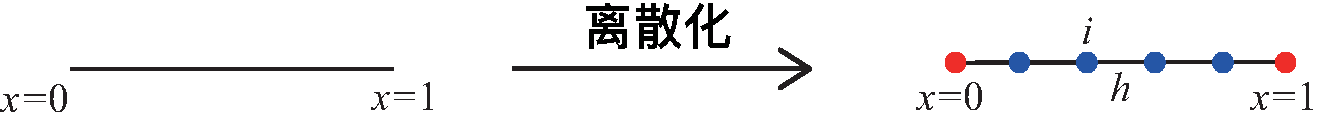
\includegraphics[width=0.6\linewidth]{pic/一维差分传热.pdf}
		\caption{一维波动计算域离散化}
		\label{一维差分波动}
	\end{figure}
	
	\item \textbf{建立离散方程}
	\begin{enumerate}[(1) ]
		\item \textbf{时间导数项}\\
		\hspace*{1em} 对目前处于第$n$个时刻的第$i$个内部节点,时间导数项二阶中心差分
		\begin{equation}
			\dfrac{u_i^{n+1}-2u_i^n+u_i^{n-1}}{(\Delta t)^2} = a^2 \dfrac{\partial^2 u}{\partial x^2}\Bigg|_i
			\label{一维波动差分时间}
		\end{equation}
		显然,当$n=0$时不存在第$-1$时刻的值,所以公式\eqref{一维波动差分时间}需要满足$n \ge 1$。所以,对于第一步的时间推进$n = 0$需要考虑初始条件所引入的差分,即二阶中心差分的另一种表示方式:
		\begin{equation}
			\dfrac{\left(\dfrac{\partial u}{\partial t}\right)^1 - \left(\dfrac{\partial u}{\partial t}\right)^0}{\Delta t} = a^2 \dfrac{\partial^2 u}{\partial x^2}\Bigg|_i 
			\quad \Rightarrow \quad
			\dfrac{\dfrac{u_1^1-u_1^0}{\Delta t} - \psi(x_i)}{\Delta t}= a^2 \dfrac{\partial^2 u}{\partial x^2}\Bigg|_i 
		\end{equation}
		可以得到第一步时间推进最终的解
		\begin{equation}
			u_i^1=\varphi(x_i)+\psi(x_i)\Delta t + a^2 (\Delta t)^2\dfrac{\partial^2 u}{\partial x^2}\Bigg|_i
		\end{equation}
		\clearpage
		
		\item \textbf{空间导数项}
		\begin{enumerate}[i. ]
			\item \textbf{显式格式}\\
			选取已知的$n$时刻
			\begin{equation}
				\begin{cases}
					\, u_i^1=\varphi(x_i)+\psi(x_i)\Delta t + a^2 (\Delta t)^2\dfrac{\varphi(x_{i+1})-2\varphi(x_i)+\varphi(x_{i-1})}{h^2}, & n = 0\\[1em]
					\,
					\dfrac{u_i^{n+1}-2u_i^n+u_i^{n-1}}{(\Delta t)^2} = a^2 \dfrac{u_{i+1}^n - 2u_i^n + u_{i-1}^n}{h^2}, & n \ge 1
				\end{cases}
			\end{equation}
			整理得
			\begin{equation}
				\bm{u}^{n+1} = \bm{B}^n
			\end{equation}
			其中,
			\begin{align}
				\bm{u}^{n+1} = 
			\begin{bmatrix}
				\, u_1^{n+1}\, \\
				\, u_2^{n+1}\, \\
				\, u_3^{n+1}\, \\
				\, u_4^{n+1}\,
			\end{bmatrix}
			\quad \quad
			\bm{B}^0 &= 
			\begin{bmatrix}
				\, \varphi(x_1)+\psi(x_1)\Delta t + a^2 (\Delta t)^2\dfrac{\varphi(x_2)-2\varphi(x_1)}{h^2} \,\\[1em]
				\, \varphi(x_2)+\psi(x_2)\Delta t + a^2 (\Delta t)^2\dfrac{\varphi(x_3)-2\varphi(x_2) + \varphi(x_1)}{h^2} \, \\[1em]
				\,  \varphi(x_3)+\psi(x_3)\Delta t + a^2 (\Delta t)^2\dfrac{\varphi(x_4)-2\varphi(x_3) + \varphi(x_2)}{h^2}  \, \\[1em]
				\, \varphi(x_4)+\psi(x_4)\Delta t + a^2 (\Delta t)^2\dfrac{-2\varphi(x_4) + \varphi(x_3)}{h^2} \, 
			\end{bmatrix}
			\\[1em]
			\bm{B}^{n}(n\ge 1)& =
			\begin{bmatrix}
				\, 2u_1^n - u_1^{n-1} + a^2(\Delta t)^2\dfrac{u_2^n-2u_1^n}{h^2}\,\\[1em]
				\,2u_2^n - u_2^{n-1} + a^2(\Delta t)^2\dfrac{u_3^n-2u_2^n+u_1^n}{h^2} \, \\[1em]
				\,  2u_3^n - u_3^{n-1} + a^2(\Delta t)^2\dfrac{u_4^n-2u_3^n + u_2^n}{h^2}  \, \\[1em]
				\, 2u_4^n - u_4^{n-1} + a^2(\Delta t)^2\dfrac{-2u_4^n+u_3^n}{h^2} \, 
			\end{bmatrix}
			\end{align}
			
			\item \textbf{隐式格式}\\
			选取待求的$n+1$时刻
			\begin{equation}
				\begin{cases}
					\, u_i^1=\varphi(x_i)+\psi(x_i)\Delta t + a^2 (\Delta t)^2\dfrac{u_{i+1}^1-2u_i^1+u_{i-1}^1}{h^2}, & n = 0\\[1em]
					\,
					\dfrac{u_i^{n+1}-2u_i^n+u_i^{n-1}}{(\Delta t)^2} = a^2 \dfrac{u_{i+1}^{n+1} - 2u_i^{n+1} + u_{i-1}^{n+1}}{h^2}, & n \ge 1
				\end{cases}
			\end{equation}
			其中,
			\begin{align}
				\bm{u}^{n+1} = 
				\begin{bmatrix}
					\, u_1^{n+1}\, \\
					\, u_2^{n+1}\, \\
					\, u_3^{n+1}\, \\
					\, u_4^{n+1}\,
				\end{bmatrix}
				\quad \quad 
				&\bm{A} =
				\begin{bmatrix}
					\, 1+\dfrac{2a^2}{h^2}(\Delta t)^2 & -\dfrac{a^2}{h^2}(\Delta t)^2 & 0 & 0\,\, \\[1em]
					\, -\dfrac{a^2}{h^2}(\Delta t)^2 & 1+\dfrac{2a^2}{h^2}(\Delta t)^2 & -\dfrac{a^2}{h^2}(\Delta t)^2 & 0 \,\, \\[1em]
					\, 0 & -\dfrac{a^2}{h^2}(\Delta t)^2 & 1+\dfrac{2a^2}{h^2}(\Delta t)^2 & -\dfrac{a^2}{h^2}(\Delta t)^2 \,\, \\[1em]
					\, 0 & 0 & -\dfrac{a^2}{h^2}(\Delta t)^2 & 1+\dfrac{2a^2}{h^2}(\Delta t)^2 \,\,
				\end{bmatrix}\\[1em]
				\bm{B}^0 &= 
				\begin{bmatrix}
					\, \varphi(x_1)+\psi(x_1)\Delta t  \,\\
					\, \varphi(x_2)+\psi(x_2)\Delta t \, \\
					\,  \varphi(x_3)+\psi(x_3)\Delta t \, \\
					\, \varphi(x_4)+\psi(x_4)\Delta t \, 
				\end{bmatrix}
				\quad \quad 
				\bm{B}^n(n\ge 1) = 
				\begin{bmatrix}
					\, 2u_1^n - u_1^{n-1} \,\\
					\,2u_2^n - u_2^{n-1} \, \\
					\,  2u_3^n - u_3^{n-1}   \, \\
					\, 2u_4^n - u_4^{n-1}  \, 
				\end{bmatrix}
			\end{align}
		\end{enumerate}
	\end{enumerate}
	\item \textbf{时间推进}
	\begin{enumerate}[(1) ]
		\item \textbf{显式格式}
		\begin{figure}[!htb]
			\centering
			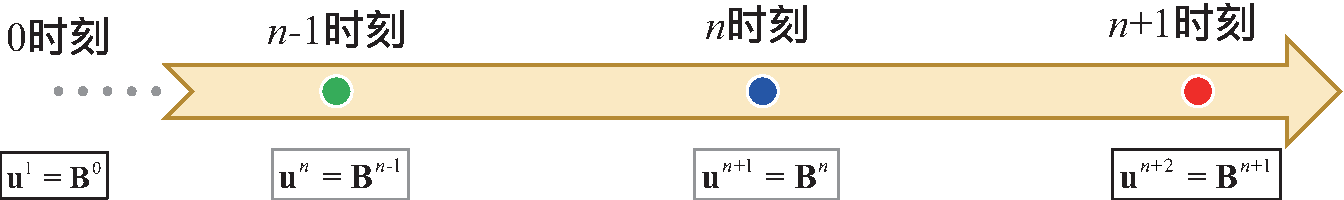
\includegraphics[width=0.7\linewidth]{pic/显式时间.pdf}
			\caption{显式格式的时间推进}
		\end{figure}
		\vspace*{-1em}
		
		\begin{itemize}
			\item $n$从0开始递增,直到$t=T$为止。
			\item 在每一时刻,只需进行代数运算获得$\bm{B}^n$便得$\bm{u}^{n+1}$,计算量小。
			\item 然而,\textcolor{red}{显式格式的时间步长要很小},否则很容易出现解振荡发散的现象。
		\end{itemize}
	
	\item \textbf{隐式格式}
	\begin{figure}[!htb]
		\centering
		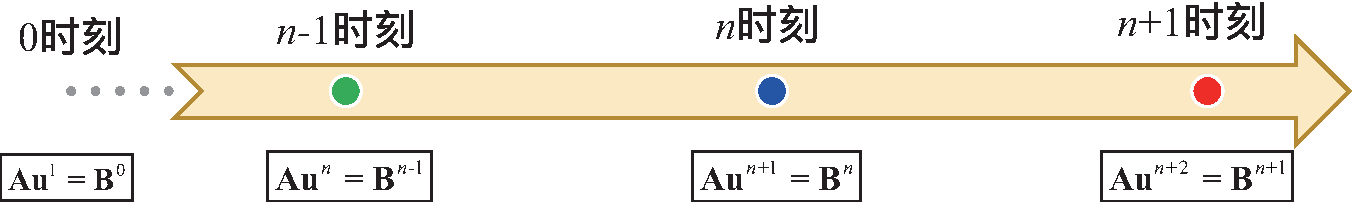
\includegraphics[width=0.7\linewidth]{pic/隐式时间.pdf}
		\caption{隐式格式的时间推进}
	\end{figure}
	\vspace*{-1em}
	
	\begin{itemize}
		\item $n$从0开始递增,直到$t=T$为止。
		\item 在每一时刻,需求解线性方程组,计算量较大。
		\item 与此同时,\textcolor{red}{允许时间更大的时间步长}。
	\end{itemize}
	\end{enumerate}
\end{enumerate}
\warn[
{
\begin{enumerate}
	\item 整体看来,与热传导方程的差分求解方法很像。
	\item 由于时间导数项变成二阶了,因此在采用二阶时间导数的中心差分时,\textcolor{red}{需要单独处理第一步时间迭代$n=0$}。
	\item 在热传导方程的求解中需要注意的事项,在这里同样需要注意。
\end{enumerate}
}
]














